
\section{Background}

%\begin{center}
%\textbf{Presenter}: \textsc{Andrew Butterfield}
%\end{center}
The project
\textit{IMA-SP Kernel Qualification – Preparation (IMAKQP)}
an  activity led by SciSys Ltd,
involving CNES, Airbus DS, TASF,
looking at the approach to be adopted for IMA-SP Separation Kernel qualification.
The activity
\textit{Formal Methods Expert to IMA-SP Kernel Qualification – Preparation
(FMEIMAKQP)}
\footnote{
   funded by ESTEC CONTRACT No. 4000112208
   supported, in part, by Science Foundation Ireland grant 13/RC/2094
}
was a parallel joint activity involving Lero@TCD,
exploring the potential role that formal verification techniques
might play in a future kernel qualification process.
It followed on from the experience of a previous activity
\textit{Method and Tools for Onboard Software Engineering (MTOBSE)}
 \footnote{
   funded by ESTEC CONTRACT No. 4000106016,
   and supported, in part, by Science Foundation Ireland grant 10/CE/I1855
}

The MTOBSE project, involving two partners in Lero: the Irish Software Research Centre,
namely the University of Limerick and Trinity College Dublin,
 looked at a top-down approach to formalising and verifying
an IMA TSP kernel,
and was reported on at two previous DASIA events\cite{MTOBSE-DASIA13,MTOBSE-DASIA13}.
We developed a reference specification for a Time-Space Partitioning (TSP) kernel\cite{MTOBSE-D03} and did a survey of formal techniques that had
potential for verifying a kernel implementation\cite{MTOBSE-D04,MTOBSE-D06}.
We then selected Isabelle/HOL\cite{NPW02} and used this to formalise the
reference specification and some of the XtratuM code\cite{MTOBSE-D07}.
We then reported on our experiences\cite{MTOBSE-D08}.
A key focus of the MTOBSE project was to consider formally verifying a kernel
to the extent required by the Common Criterion (CC) guidelines for both functional correctness and security\cite{RD-07},
with particular reference to the Separation Kernel Protection Profile (SKPP)\cite{RD-08}.

The focus of FMEIMAKQP was exploring approaches for qualifying
an \emph{existing} separation kernel implementation as its starting point.
In particular,
the focus was on functional correctness rather than security properties.
From a formal perspective this involved looking much more closely at techniques
for reasoning at or close to source code level.
Also of interest was to explore how formal techniques might best be integrated
with well-established software engineering practises,
such as testing, and model-based development.
Results of this activity
were reported at DASIA in 2015 \cite{FMEIMAKQP-DASIA15},
and in 2016 \cite{FMEIMAKQP-DASIA16}.

\section{Key FMEIMAKQP Outcomes}
Key formal-methods results in the Final Report for FMEIMAKQP\cite{FMEIMAKQP-R1}
where:
\begin{enumerate}
  \item
    A High-Level model written in CSP\cite{hoare-1985:commuseque:}
    of the Leon-processor based platform,
    and some of the Requirement Baseline\cite{IMAKQP-D02}
    behavioural specifications.
    Analysis of these models was done using
    the model/refinement checking tool FDR\cite{FDR3}.
    Some of this reported on work done in Trinity College Dublin
    for a Masters Thesis\cite{KH-MCS2016}
  \item
    The use of the Frama-C toolkit\cite{Frama-C:user:Magnesium} to add low-level
    annotations to the C sources for the Xtratum hypervisor\cite{CRM10}.
\end{enumerate}
A key issue that has to be addressed for both of these results
was the fact that they involved a consideration of ``unavoidable concurreny'',
along with the non-determinism that usually arises.
% The purpose of the separation kernel is to allow multiple
% (software) partitions to run on one hardware platform,
% each being isolated in both time and space,
% with any cross-communication limited to what is authorised.
For a single-core system, despite the fact that at any point in time,
we have only one partition or the kernel itself actually running,
we find that we have what is an essentially \emph{concurrent} system.
The CPU executes instruction in a sequential manner,
but also running concurrently is the MMU/MPU which monitors the bus traffic,
as well as the interrupt request hardware.

Key formal methods-related recommendations in \cite{FMEIMAKQP-R1} include:
\begin{itemize}
  \item
    Formalising the Requirements Baseline\\
    It would describe a relationship between a valid kernel configuration
    and the permissible behaviours associated
    with both the kernel and all the partitions defined in the configuration.
    The primary value of this model
    is that it would provide a way to check the requirements
    baseline for internal consistency.
  \item
    Formalising the Data Invariant\\
    A configuration invariant would allow the formal verification
    of configuration tools.
    It could also be used to verify the correct use by the kernel of its
    own internal data-structures.
  \item
    Verifying \textbf{PK-9}\\
    This is a requirement regarding the correct save/restore of partition state
    as a result of context-switches.
    It proved difficult to test adequately.
  \item
    Completing the CSP models\\
    This work \cite{KH-MCS2016} was very much a proof of concept.
    But is has potential to do much more,
    particularly because CSP's model of events and concurrency
    is a good fit to the concurrent behaviour of the kernel platforms,
    and the general behavioural flavour of many of the requirements..
\end{itemize}
We also suggested other kinds of space-related modelling and software
activities that might benefit from early formal modelling:
e.g. SAVOIR (architecture,specifications,data models,interfaces, protocols).

The last recommendation discussed various modalities
for future activities in this space.
In particular it was noted that student projects
are a way to conduct explorations of various ideas,
as demonstrated by the work reported at DASIA 2016.

In the sequel,
we shall take requirement PK-230 from IMAKQP-D02\cite{IMAKQP-D02}
as a running example:
\begin{quote}
PK-230: \textit{\textbf{Partitions shall be executed in user mode.}}
\end{quote}

\section{Revising the CSP Model}

We have been reworking the CSP models described in \cite{KH-MCS2016}
mainly to try to avoid the problem of ``combinatorial state-space explosion''
that bedevils model-checking based techniques.
There are two lines of attack we are bringing to bear on this problem:
\begin{enumerate}
  \item Abstraction:
   In order to be able to successfully run checks,
   we need to take particular care to abstract away from all irrelevent
   aspects of system state.
   For example, in order to model how the MMU monitors memory accesses
   and how the kernel configures the MMU and handles its interrupts,
   we probably don't need to distinguish between reads/writes,
   or the specific data values, at least for many requirements.
   The challenge is finding the greatest abstraction that does not lose  information
   that is in fact important for the requirement or behaviour being modelled.
  \item Modularity:
    The verification approach is to take a model of the Kernel, some Partitions,
    and the Hardware Platform (KPHP),
    and construct a way to use the requirement model
    to act as a monitor for the kernel behaviour.
    With CSP it is possible to build individual models for each of (most of)
    the baseline requirements
    This makes it possible to check each requirement individually,
    which is clearly a very useful aspect of this modelling approach.
    However much of this advantage is lost if a check for a given requirement
    fails because of state-space explosions
    due to parts of the KPHP state
    that are irrelevant to that given requirement.
    We are exploring how to factor the various models into sub-models
    that focus on key subsets of the overall space,
    so that each requirement check is tailored to only use the relevant subset.
\end{enumerate}

\subsection{Modelling the Environment}

We consider the ``environment'' to be the platform and software entities
over which we hope to see the requirements being enacted.
We have adopted a view that we have ``Processes''
that engage in ``Events''. Events are observable indivisible actions,
that can be simple synchronisation events,
or have associated data, in which case they behave like messages.
A Process is is a set of ``behaviours'',
with each behaviour having two aspects:
a history of past events we have observed, known as a ``trace'',
and a record of those events that the process is currently willing to perform.
Any given process, or set of behaviours, can also be modelled as a state machine.
An observed event causes a transition from the current state to a next state,
and the current state only allows certain transitions.
The CSP language is defined on top of this conceptual model of processes, states
and behaviours.


As part of the environment,
we have the hardware platform on which the kernel will run.
We need to model hardware that runs concurrently,
including the CPU, memory, MPU, and interrupt handling.
The observable events of interest include memory-bus activity,
interrupt signals, processor status and modes, etc.,
depending on specific requirements.

For PK-230, we are particularly interested in the processor's
execution privilege level,
which can be either ``User'', or ``Supervisor''.

However, the hardware model isn't enough.
We also need to model abstract kernel entities, some being software,
others including data, and abstract kernel-related events.
We need to distinguish the kernel software from that of the partitions,
be able to observe configuration and schedule data,
and discuss events such as starting or stopping a partition,
or hypercalls requested by a partition.
This is necessary, because the requirements mention these concepts.

For PK-230, we are required to ensure that when any partition code
is being executed, that the processor is only running at the User
privilege level.

We need to use a considerable degree of abstraction
to keep model-checking tractable.
For the platform model, we have to answer questions such as:
how many distinct addressess? data values? intructions? interrupt levels?
Representing just one byte involves 256 states,
and its contribution to the total state-space is obtained by multiplying
its state-count with the number of other states.
What this all leads to is the need to use the smallest number of different
values required to produce an ``adequate'' model.
We also note that the various requirements are interested in different
things, so we may want to tailor the model of any given aspect
in a specific way for each requirement.

For PK-230, we need to be able to observe the CPU mode,
and the current instruction address.
A violation results if we observe an instruction fetch from an address
associated with partition code, while the processor is in suerpvisor mode.
All we need to be able to distinguish,
in order to be able to assert compliance with, or a violation of, PK-230,
is the CPU mode (User/Suervisor) and the abstract entity (kernel/partition)
to which the current instruction address belongs.

\subsection{CSP Model for PK-230}

We present here some fragments of the CSP model developed for PK-230
and some of the other ``Partition Management'' requirements.

We propose three entities: kernel and two partitions:
\begin{cspm}
datatype ENT = KNL | P1 | P2
\end{cspm}
We define three machine instructions: generic (NOP),
and two to reset(S0)/set(S1)
the processor privilege mode.
We also introduce a 1-bit instruction operand.
\begin{cspm}
datatype I = NOP | S0 | S1
nametype OP = {0..1}
\end{cspm}
We now define an observable instruction fetch as an entity/instruction/opcode
triple, tagged as a fetched instruction:
\begin{cspm}
channel fi : ENT.I.OP
\end{cspm}
The channel keyword in CSP introduces a visible event,
in this case structured as a channel ``name'' (fi)
and three data components.

We want to make processor mode changes observable:
\begin{cspm}
datatype PM = USR | SUP
channel pm : PM
\end{cspm}
We can then model the platform, tailored for partition management:
\begin{cspm}
PMM = pm.SUP -> PMMRUN -- start in SUP mode
PMMRUN =  fi?ent.S1?op    -> pm.SUP -> PMMRUN
       [] fi?ent.S0?op    -> pm.USR -> PMMRUN
       [] fi?ent.NOP?op             -> PMMRUN
       [] hc?p?call:HCALL -> pm.SUP -> PMMRUN
\end{cspm}
The notation \verb"a -> P" denotes a process that will perform event \texttt{a},
and then behave like process \texttt{P}.
The notation \verb"a -> P [] b -> Q" is a process
that offers the environment the choice between events \texttt{a} and \texttt{b}.
Once the environment chooses, and the event takes place, then this process
will behave like \texttt{P}, if \texttt{a} was performed, otherwise like \texttt{Q}.
An event notation of the form \texttt{c?x -> P(x)}, where \texttt{x} is a variable,
is syntactic sugar for
a choice over events of the form \texttt{c.k}, where \texttt{k} ranges
over all values that \texttt{x} can take. Once \texttt{k} has been determined by the environment, then the resulting behavior is that of \texttt{P(k)}.
This models the platform responding to instructions, and using \texttt{pm} to signal when the processor mode has changed.
This occurs from instructions \texttt{S1} and \texttt{S0}. as well as hypercalls (interrupts).
The model is not totally faithful, as it allows the processor to execute \texttt{S1}
while in user mode, which is not allowed
---such a model is easily developed, but we omit details for brevity.
The PMM model does not act as an ``enforcer'' of any requirement,
but simply shows what the platform will do under the relevant circumstances.
The role of enforcing PK-230 will be carried out by a specific CSP process:
\begin{cspm}
channel pk230fail -- for signalling violation
PK230 = PK230sup -- SUP mode to start
PK230sup =  fi.P1?i?op  -> pk230fail -> STOP
         [] fi.KNL?i?op -> PK230sup
         [] pm.USR      -> PK230usr -- switch mode
         [] pm.SUP      -> PK230sup
PK230usr =  fi?ent?i?op -> PK230usr
         [] pm.USR      -> PK230usr
         [] pm.SUP      -> PK230sup -- switch mode
\end{cspm}
We have two processes defined here---one captures behaviour in supervisor
mode, the other that of user mode. This process runs almost forever,
the one exception being when it is in supervisor mode, and detects
any instruction (\texttt{?i?op}) being executed by a partition (\texttt{P1}).
In this case it signals a failure and then deliberately deadlocks (\texttt{STOP}).

We can put these processes in parallel, with a third non-stop process modelling actual kernel and partition code, requiring them to agree on all these events.
In this model, the only source of deadlock is the first line of \texttt{PK230sup}.
Hence, we can use the deadlock freedom check of FDR as a way to check for complaince
with PK230.




\section{A Requirements DSL}

The approach of tailoring CSP models by hand to model requirements
is very ad-hoc, and kernel specific.
Of interest are ways to generalise this approach to we can more easily
cover a wider range of requirements,
even going beyoind the separation kernel domain.
An idea we decided to explore,
as a student project\cite{Costelloe17},
was the development
of a Domain-Specific Language (DSL) to assist in capture requirements
in a machine-readable and processable form.
Such a language could then be used to develop tools to
perform requirements consistency checking,
and to connect the requirement to other modelling notations and techniques.

We proposed to implement the DSL using the functional programming language
Haskell (www.haskell.org).
This is because DSL development is something for which that language is ideally suited.
The concrete language syntax is that of Haskell,
so no parsers need be written.
The language elements can be defined as atomic building blocks
used in conjunction with combining forms, using the type-class system
of Haskell.
This leverages the type system to ensure descriptions are well-formed,
but does not impose any \emph{a-priori} semantics on the language.
The class system is enacted by defining various
datatypes that do have semantic significance,
and showing how they are instances of the DSL language.
This means we can easily give the same description multiple meanings.
Such meanings could comprise:
\begin{itemize}
  \item A Natural Language (NL) text rendering --- useful for review of the requirements
  \item CSP Output --- so we can exploit the CSP models and the FDR model-checker.
  \item Structure Graphs --- tailored for some kind of consistency/completness checking
  \item Simulator Output --- generate something for an appropriate simulation tool.
\end{itemize}
\begin{figure}
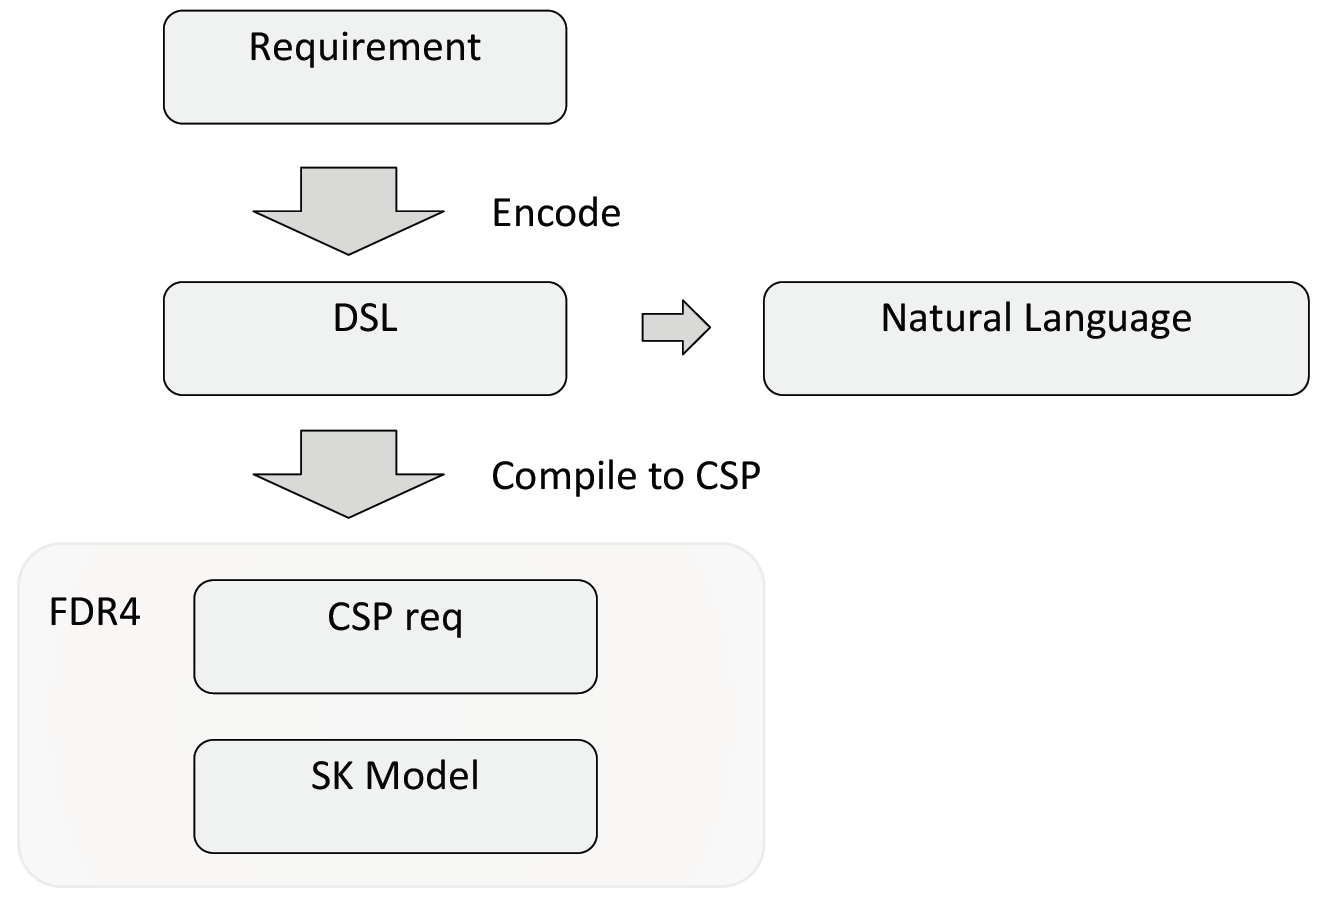
\includegraphics[scale=0.35]{images/CC-1-1-Project-Design}
  \caption{Reqmts DSL Usage, from \cite{Costelloe17}}
\end{figure}
DSL development is non-tricial,
and the key challenge is the correct identification
of the atomic building blocks and combining forms.
The first attempt to explore such a language was done by taking a broad
sample of requirements from different parts of the IMAKQP-D02.
This did not prove to be too succesful,
as each requirememt looked very ``unique'',
and it was hard to find common aspects.

A second attempt decided to select requirements from a cognate area,
so it was decided to focus on those involved in ``Partition Management''.
This made it easier to find more commonality,
at the risk of being too specific.
At this point we were able to identify some common requirement ``idioms'',
most notably: ``May ..'', ``Must'' and ``Must Not ..''.
In Haskell:
\begin{code}
data Requirement
 = Allowed Actor Action Situation String
 | Forbidden Actor Action Situation String
 | Must Actor Action Situation String
\end{code}
We have a mix of generic concepts,
and very application-specific ones, as evidenced by the definitions
of \texttt{Actor} and \texttt{Situation}:
\begin{code}
data Actor = Kernel | Act Partition
           | SchedulingPlan | Configuration
data Situation
 = Initialisation
 | Transition PartitionTransition
 | Always | After Situation | Before Situation
\end{code}
Given the above definitions, plus a few more omitted for lack of space,
we can then encode PK-230 as:
\begin{code}
pk230 =
 Must (Act Partition)
      (Assert ((PriviledgeOf Partition)
               `Equ`
               (Const User)))
      Always
      "pk230"
\end{code}
This can then be rendered to natural language as
\begin{quote}
``the Partition must have Partition's priviledge equal to User''
\end{quote}
A haskell module was then developed to map requirement concepts
as found in the DSL into a semantic model of processes and events,
based on the notion of states with events triggering transitions between states.
This is then used to generate CSP---the code shown earlier for \texttt{PK230} was generated this way.

\subsection{Conclusions}

We have done some exploration into an emerging framework for handling kernel
requirements,
that we hope will also generalised beyond this application area.
At present we have only encoded partition managememt requirements,
so we need to validate this approach by considering a broader range.
We are keeping things very modular, with very specific targetted platform models.
We have a model tailored for partition management, but we will need others
for FDIR, interrupts, scheduling, etc.
A big issue we will have to address is how to keep all these tailored models
consistent with each other.
The ultimate goal is to be able to deduce an abstract seperation kernel
\emph{specification} from all the kernel code models that satisfy the requirememt models.
